\documentclass[a4paper,12pt]{article}
\usepackage[utf8x]{inputenc}
\usepackage{amssymb}
\usepackage{amsfonts}
\usepackage{mathrsfs}
\usepackage{amsmath}
\usepackage{amsthm}
\usepackage[margin=3cm]{geometry}
\usepackage{times}
\usepackage{graphicx}
\usepackage{enumitem}
\usepackage{fancyhdr}
\usepackage{hyperref}
\usepackage{setspace}
\usepackage{subcaption}
\usepackage{mathtools}

\pagestyle{fancy}
\fancyhf{}
\lhead{Thomas Delaney}
\rhead{Fluorescence Modelling}
\cfoot{\thepage}

\newtheorem{theorem}{Theorem}
\newtheorem{proposition}{Proposition}[section]
\newtheorem{lemma}{Lemma}[section]
\newtheorem{corollary}{Corollary}[section]
\theoremstyle{definition}
\newtheorem{definition}{Definition}[section]

\newcommand{\boldnabla}{\mbox{\boldmath$\nabla$}} % to be used in mathmode
\newcommand{\cbar}{\overline{\mathbb{C}}}% to be used in mathmode
\newcommand{\diff}[2]{\frac{d #1}{d #2}}% to be used in mathmode
\newcommand{\difff}[2]{\frac{d^2 #1}{d #2^2}}% to be used in mathmode
\newcommand{\pdiff}[2]{\frac{\partial #1}{\partial #2}} % to be used in mathmode
\newcommand{\pdifff}[2]{\frac{\partial^2 #1}{\partial #2^2}}% to be used in mathmode
\newcommand{\upperth}{$^{\mbox{\footnotesize{th}}}$}%to be used in text mode
\newcommand{\vect}[1]{\mathbf{#1}}% to be used in mathmode
\newcommand{\curl}[1]{\boldnabla \times \vect{#1}} % to be used in mathmode
\newcommand{\divr}[1]{\boldnabla \cdot \vect{#1}} %to be used in mathmode
\newcommand{\modu}[1]{\left| #1 \right|} %to be used in mathmode
\newcommand{\brak}[1]{\left( #1 \right)} % to be used in mathmode
\newcommand{\comm}[2]{\left[ #1 , #2 \right]} %to be used in mathmode
\newcommand{\dop}{\vect{d}} %to be used in mathmode
\newcommand{\cov}{\text{cov}} %to be used in mathmode
\newcommand{\var}{\text{var}} %to be used in mathmode
\newcommand{\mb}{\mathbf} %to be used in mathmode
\newcommand{\bs}{\boldsymbol} %to be used in mathmode
% Title Page
\title{Modelling the fluorescence produced by fluorescent calcium indicators in response to sequences of action potentials}
\date{}
\author{Thomas J. Delaney \\ Cian O'Donnell, Michael C. Ashby}

\begin{document}

\maketitle

\newpage

\abstract{The use of fluorescent calcium indicators, such as GCaMP6s, to monitor neuronal activity is widespread. But the relationship between the fluorescence signal and action potential firing is poorly understood. Furthermore, the effects of the indicator characteristics on this fluorescence signal are unknown. For example, it is known that genetically encoded indicators accumulate within neurons over weeks and months. This makes comparison of activity levels at different time points difficult. As a result, whether or not spike train inference is always possible using fluorescent calcium indicators remains unknown.

The aim of this project was to model the fluorescence traces produced by a fluorescent calcium indicator in a neuron soma, given parameters such as binding rate, dissociation rate, and molecular concentration from a specific spike train. The ultimate goal of the model is to allow benchmarking of the various spike inference algorithms that have been developed, and to understand how indicator characteristics affect the quality of spike train inference.

The modelled cell contents consisted of free calcium, fluorescent indicator molecules, and mobile and immobile endogenous calcium buffers. The indicator molecules which were bound to a calcium molecule could be either excited, i.e. able to release a photon, or relaxed. In order to reproduce the noise in the system dynamics, we modelled the release of photons from the excited indicator bound calcium as a stochastic process.

The fluorescence traces produced by the simulation were calibrated to reproduce the signal-to-noise ratio observed in experimental data. Spike inference algorithms were used to infer spike trains from the experimental fluorescence traces and the modelled fluorescence traces. The parameters of the model were then varied in order to determine the effect on the system dynamics and the effects on spike inference.} % no citations in the abstract

\newpage

\tableofcontents

\newpage

\section{Calcium Imaging}

\begin{figure}[p]
  \begin{subfigure}{0.5\textwidth}
    \centering
    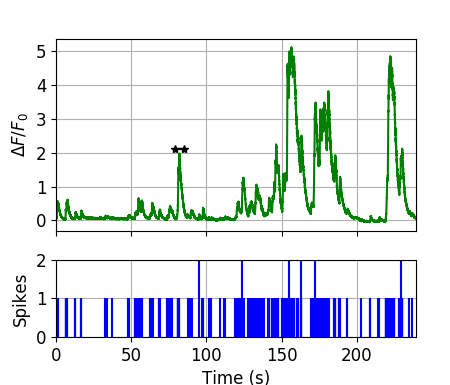
\includegraphics[width=\textwidth]{figures/spike_finder_example_8.png}
    \caption{}
  \end{subfigure}
  \begin{subfigure}{0.5\textwidth}
    \centering
    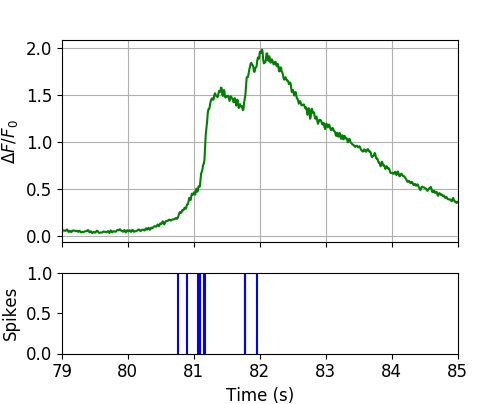
\includegraphics[width=\textwidth]{figures/spike_finder_example_8_zoomed.png}
    \caption{}
  \end{subfigure}
  \caption{(a) Plot of a spike train and the corresponding GCaMP6s fluorescence trace. Data courtesy of spikefinder.codeneuro.org (b) The same image as (a) but zoomed into the period from 79s to 85s. This period is marked on figure (a) by the horizontal black line with stars at each end. A group of six action potentials around the 81s point followed by a group of three action potentials just before the 82s point are shown. The decay of the fluorescence trace is much slower than the dynamics of an action potential.}
  \label{fig:spike_finder_example}
\end{figure}

\section{Results}

\subsection{The model}

\begin{figure}[p]
  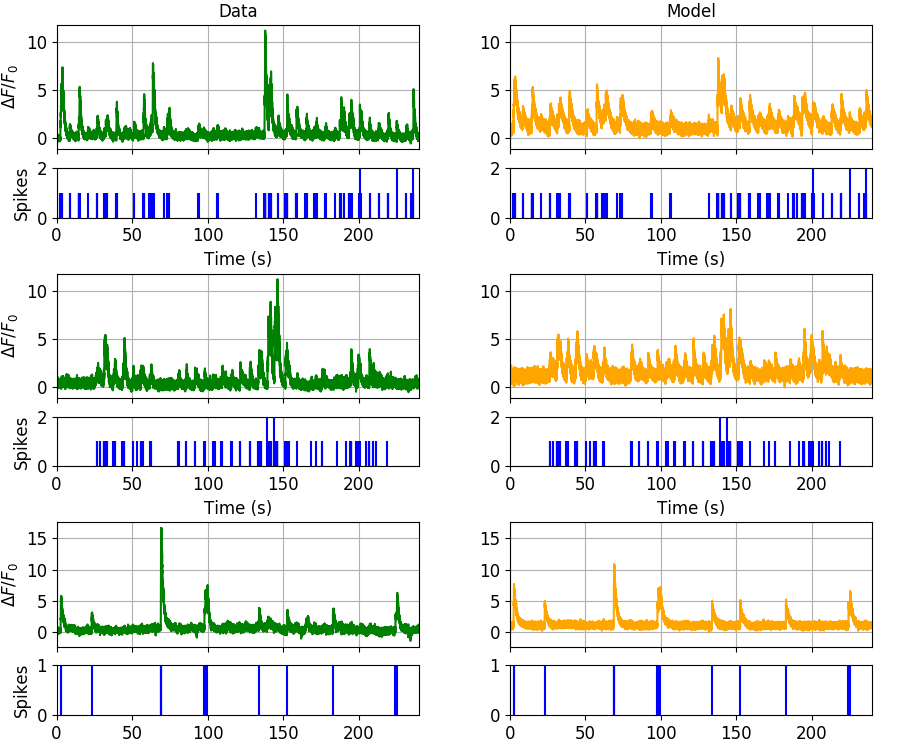
\includegraphics[width=\textwidth]{figures/trace_comparison.png}
  \caption{(LHS) Observed fluorescence traces from the Spikefinder dataset with their associated spike trains. (RHS) Fluorescence traces created by the model given the same spike trains. Traces were created after the model was optimised for each florescence trace.}
  \label{fig:observed_modelled_examples}
\end{figure}

\begin{figure}
  \begin{subfigure}{0.5\textwidth}
    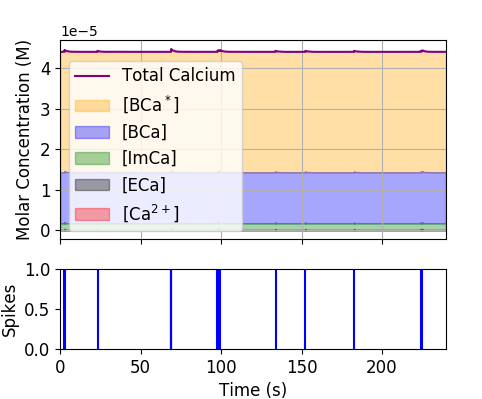
\includegraphics[width=\textwidth]{figures/concentration_dynamics.png}
    \caption{}
    \label{fig:contrentration_dynamics}
  \end{subfigure}
  \begin{subfigure}{0.5\textwidth}
    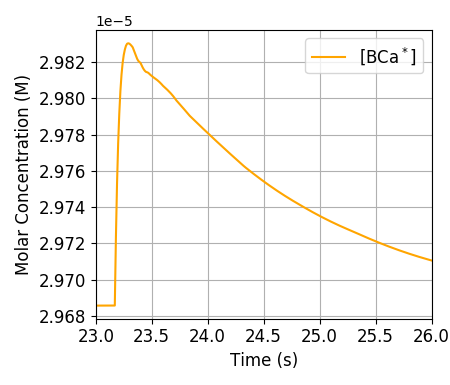
\includegraphics[width=\textwidth]{figures/concentration_dynamics_18_zoomed_BCa_star.png}
    \caption{}
  \end{subfigure}
  \begin{subfigure}{0.5\textwidth}
    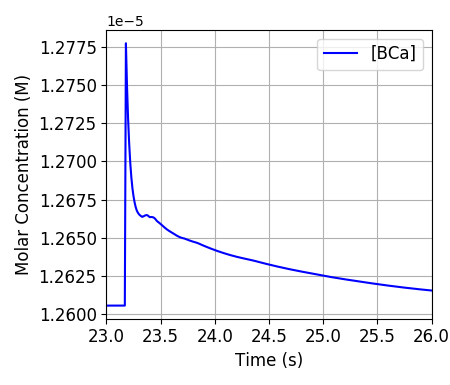
\includegraphics[width=\textwidth]{figures/concentration_dynamics_18_zoomed_BCa.png}
    \caption{}
  \end{subfigure}
  \begin{subfigure}{0.5\textwidth}
    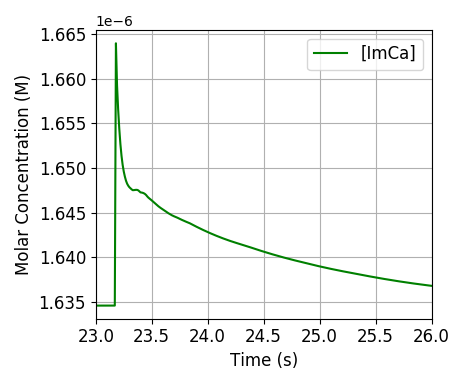
\includegraphics[width=\textwidth]{figures/concentration_dynamics_18_zoomed_ImCa.png}
    \caption{}
  \end{subfigure}
  \begin{subfigure}{0.5\textwidth}
    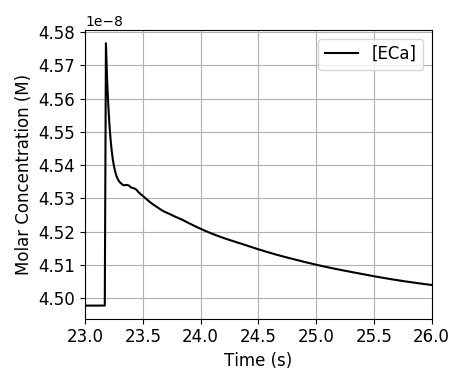
\includegraphics[width=\textwidth]{figures/concentration_dynamics_18_zoomed_ECa.png}
    \caption{}
  \end{subfigure}
  \begin{subfigure}{0.5\textwidth}
    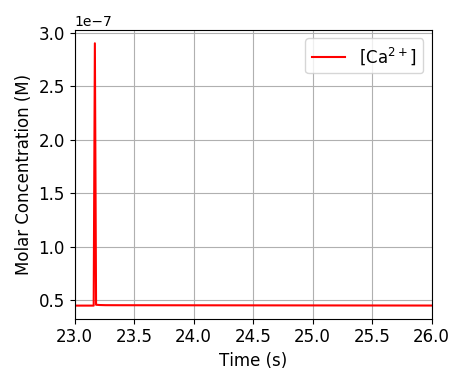
\includegraphics[width=\textwidth]{figures/concentration_dynamics_18_zoomed_Ca.png}
    \caption{}
  \end{subfigure}
  \caption{\textbf{Calcium Buffering Dynamics } (a) The proportions of bound and free calcium concentrations within a cell, with the associated spike train. (b)-(f) The dynamics of the concentration of (b) excited indicator bound calcium, (c) indicator bound calcium, (d) immobile endogeneous buffer bound calcium, (e) mobile endogeneous buffer bound calcium, and (f) free calcium in response to an action potential at 23.17s.}
  \label{fig:concentrations}
\end{figure}

\subsection{Spike Inference}

\begin{figure}
  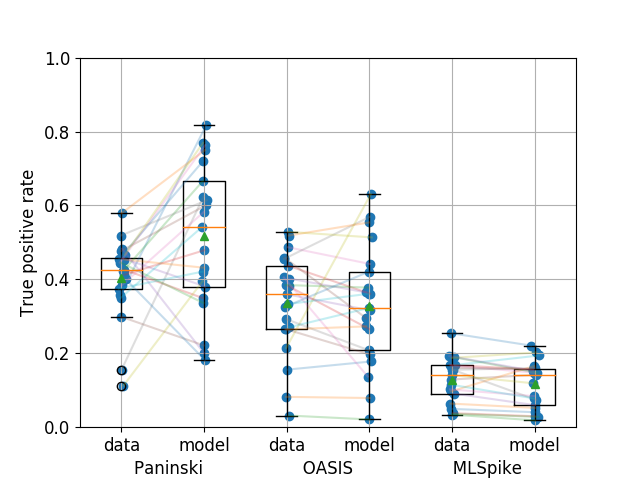
\includegraphics[width=\textwidth]{figures/three_algo_comparison_tp_paper.png}
  \caption{Box plots showing the distribution of the true positive rates achieved by three spike inference algorithms when applied to observed spike trains, and modelled spike trains. Data points overlaid as blue circles. The performance is similar from real and simulated data for each of the algorithms.}
  \label{fig:three_algo_comparison}
\end{figure}

\subsection{Perturbation analysis}

\subsubsection{Perturbing indicator concentration}

\begin{figure}
  \begin{subfigure}{\textwidth}
	   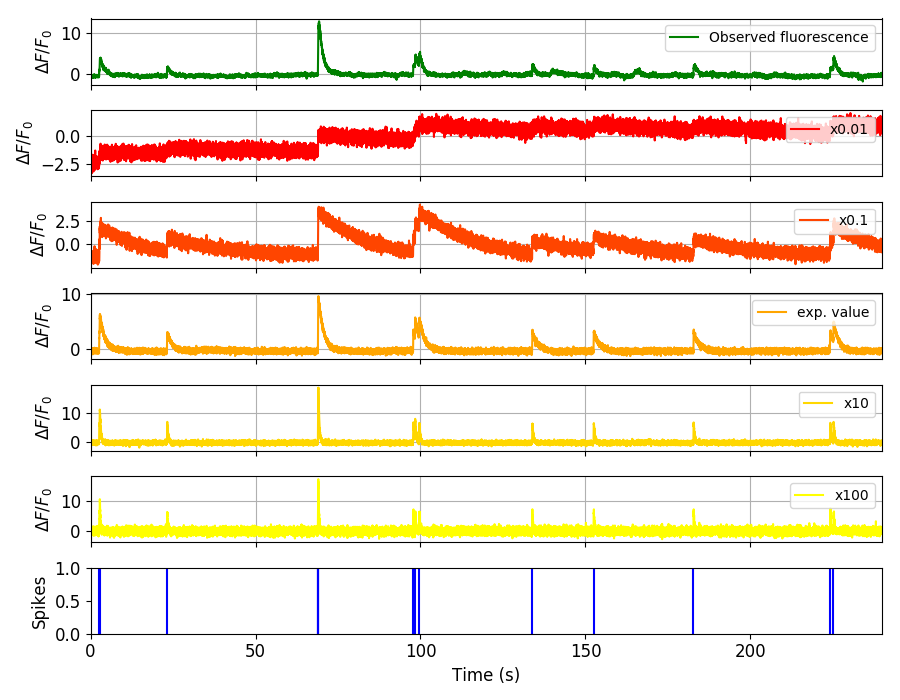
\includegraphics[width=\linewidth]{figures/indicator_perturbed_fluorescence_18_paper.png}
     \caption{}
  \end{subfigure}
  \begin{subfigure}{0.5\textwidth}
	   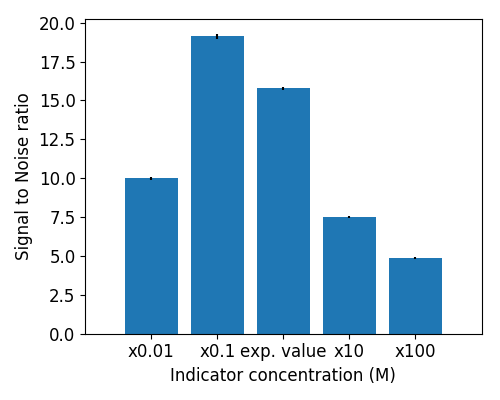
\includegraphics[width=\linewidth]{figures/indicator_perturbed_snr.png}
     \caption{}
  \end{subfigure}
  \begin{subfigure}{0.5\textwidth}
	   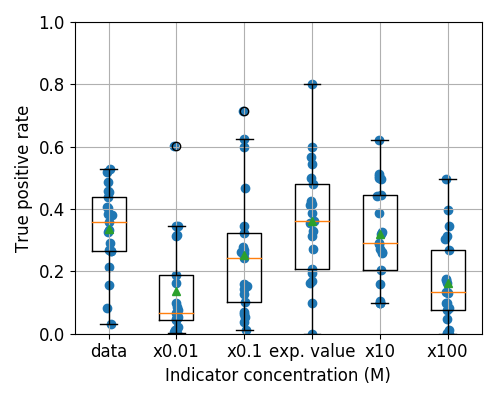
\includegraphics[width=\linewidth]{figures/indictor_perturbed_oasis_first_paper.png}
     \caption{}
  \end{subfigure}
  \caption{(a) An example trace for each of the five perturbed values for the concentration of fluorescent calcium indicator. The top two traces are produced by the lower perturbed values, the middle trace is produced by the experimental value, and the lowest two traces are produced when using the higher perturbed values. (b) The signal-to-noise ratio of the modelled fluorescence traces using each of the four perturbed values, and the experimental value. Extreme perturbations of the concentration either above or below the experimental level lowered the SNR. (c) The true-positive rates of the deconvolution algorithm's predictions when inferring from the observed data, and inferring from modelled traces using the perturbed and experimental values. We found that the algorithms performs equally badly on the two most extreme values, and performs equally well on the experimental value, and the next higher perturbed value.}
  \label{fig:indicator_perturbed}
\end{figure}

\subsubsection{Perturbing immobile endogeneous buffer concentration}

\begin{figure}
  \begin{subfigure}{\textwidth}
	   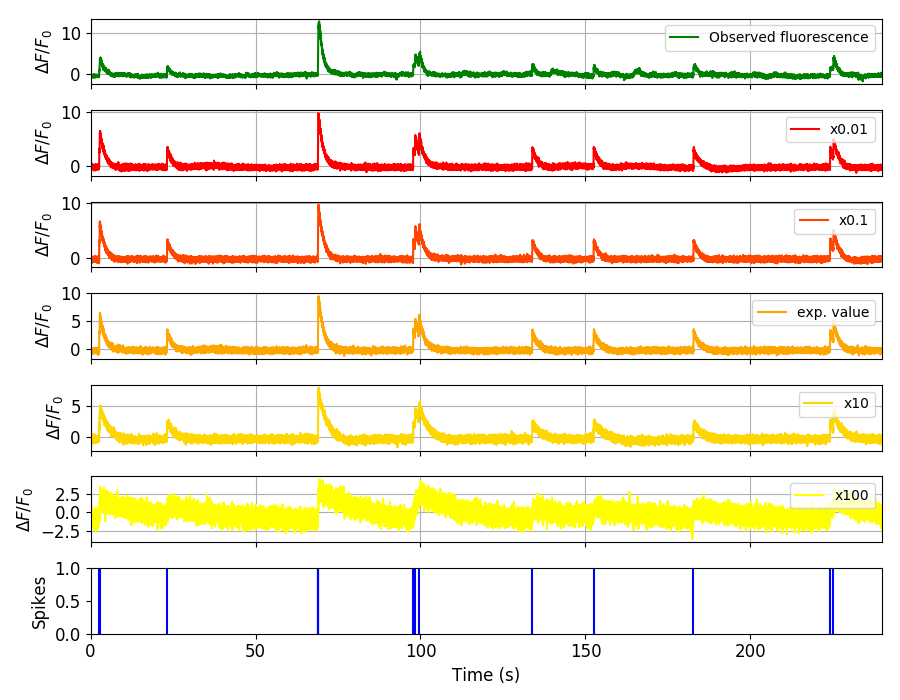
\includegraphics[width=\linewidth]{figures/immobile_perturbed_fluorescence_18_paper.png}
     \caption{}
  \end{subfigure}
  \begin{subfigure}{0.5\textwidth}
	   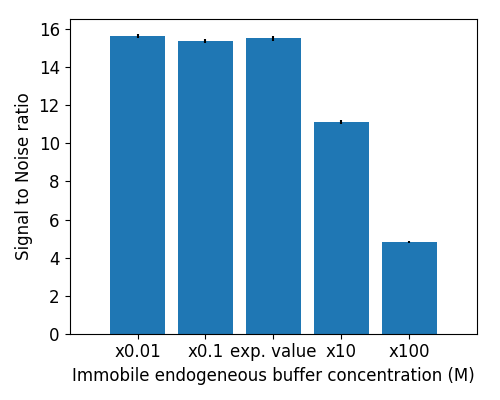
\includegraphics[width=\linewidth]{figures/immobile_perturbed_snr.png}
     \caption{}
  \end{subfigure}
  \begin{subfigure}{0.5\textwidth}
	   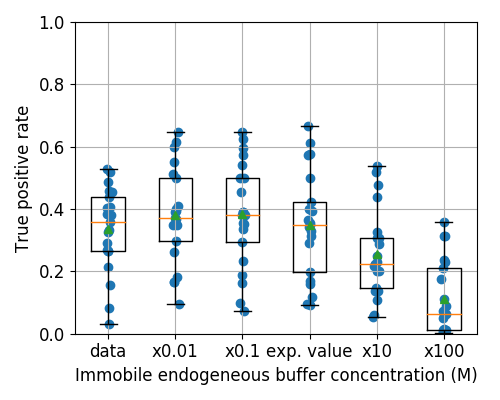
\includegraphics[width=\linewidth]{figures/immobile_perturbed_oasis_first_paper.png}
     \caption{}
  \end{subfigure}
  \caption{(a) An example trace for each of the five perturbed values for the concentration of immobile endogeneous buffer.	(b) The signal-to-noise ratio of the modelled fluorescence traces using each of the four perturbed values, and the experimental value. The lower values for the immobile buffer produce the same SNR as the experimental value. But the higher perturbed values produce fluorescence traces with a lower SNR.	(c) The true-positive rates of the deconvolution algorithm's predictions when inferring from the observed data, and inferring from modelled traces using the perturbed and experimental values.}
  \label{fig:endogeneous_perturbed}
\end{figure}

\subsubsection{Perturbing indicator binding and unbinding rates}

\begin{figure}
  \begin{subfigure}{\textwidth}
	   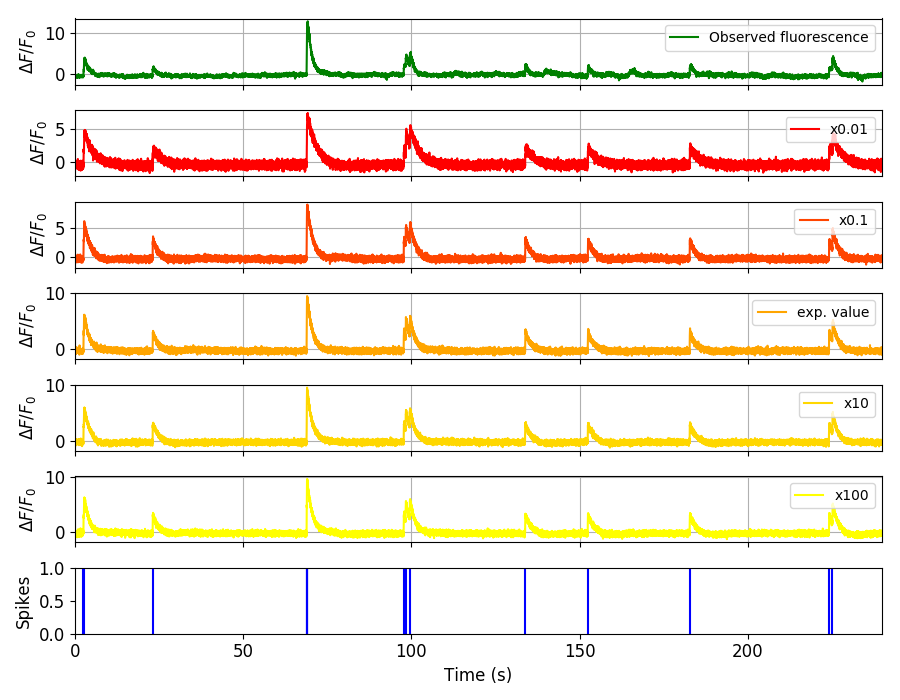
\includegraphics[width=\linewidth]{figures/b_i_f_i_perturbed_fluorescence_18_paper.png}
     \caption{}
  \end{subfigure}
  \begin{subfigure}{0.5\textwidth}
	   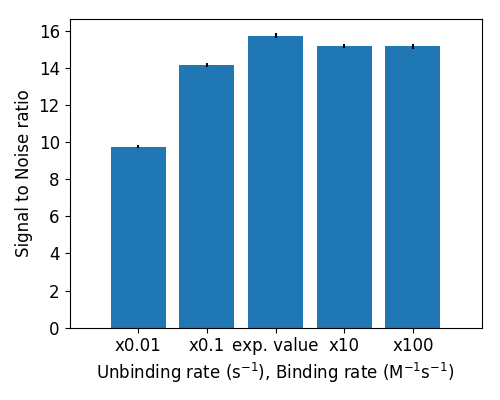
\includegraphics[width=\linewidth]{figures/b_i_f_i_perturbed_snr.png}
     \caption{}
  \end{subfigure}
  \begin{subfigure}{0.5\textwidth}
	   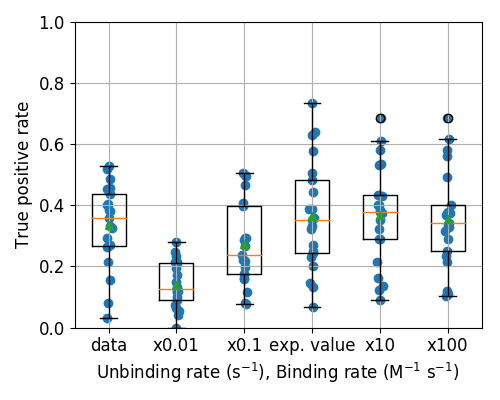
\includegraphics[width=\linewidth]{figures/b_i_f_i_perturbed_oasis_tp_paper.png}
     \caption{}
  \end{subfigure}
  \caption{(a) An example trace for each of the five pairs of values used for the binding and unbinding rates of the fluorescent calcium indicator. (b) The signal-to-noise ratio of the modelled fluorescence traces using each of the four perturbed values, and the experimental value. The SNRs for the two pairs with values lower than the experimental value are lower than the experimental pair or the higher value pairs. (c) The true-positive rates of the deconvolution algorithm's predictions when inferring from the observed data, and inferring from modelled traces using the perturbed and experimental values.}
  \label{fig:rates_perturbed}
\end{figure}

\subsection{Varying spike rate for different cell types}

\begin{figure}
  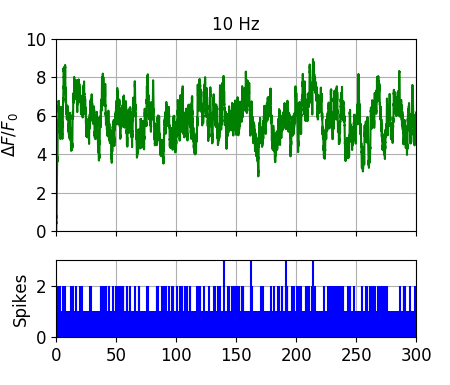
\includegraphics[width=0.329\linewidth]{figures/freq_compare_images_10_Hz_1_1.png}
  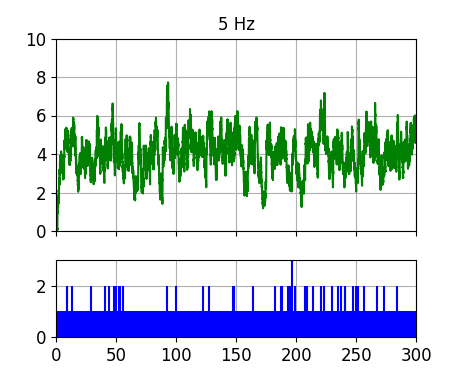
\includegraphics[width=0.329\linewidth]{figures/freq_compare_images_5_Hz_1_2.png}
  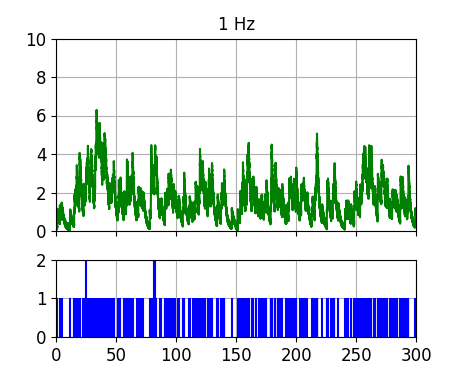
\includegraphics[width=0.329\linewidth]{figures/freq_compare_images_1_Hz_1_3.png}
  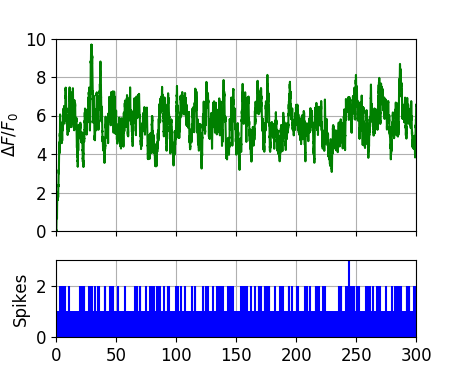
\includegraphics[width=0.329\linewidth]{figures/freq_compare_images_10_Hz_2_4.png}
  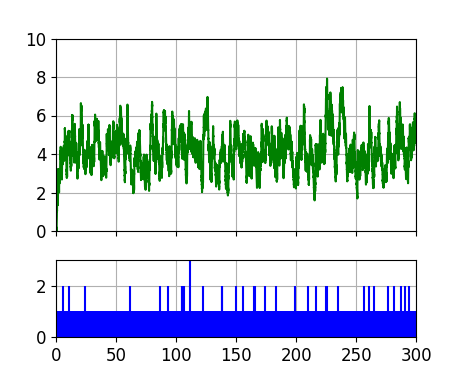
\includegraphics[width=0.329\linewidth]{figures/freq_compare_images_5_Hz_2_5.png}
  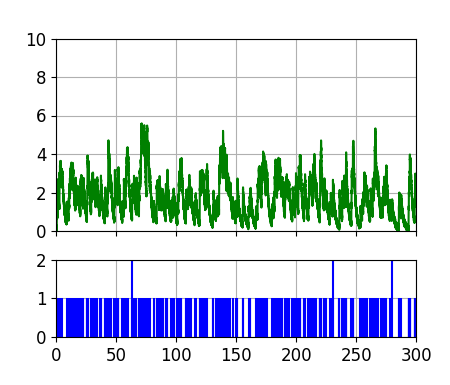
\includegraphics[width=0.329\linewidth]{figures/freq_compare_images_1_Hz_2_6.png}
  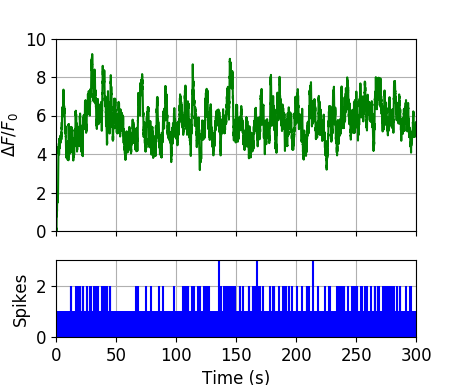
\includegraphics[width=0.329\linewidth]{figures/freq_compare_images_10_Hz_3_7.png}
  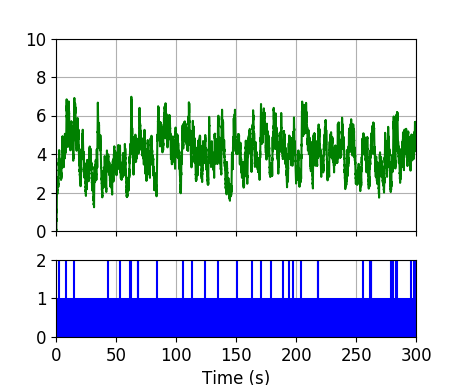
\includegraphics[width=0.329\linewidth]{figures/freq_compare_images_5_Hz_3_8.png}
  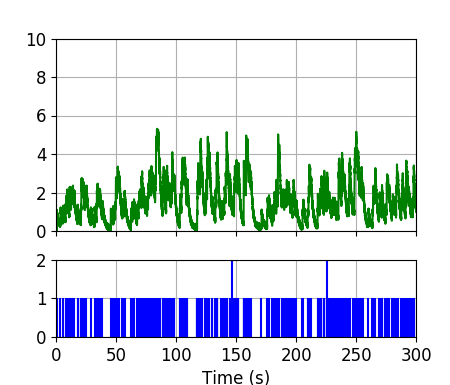
\includegraphics[width=0.329\linewidth]{figures/freq_compare_images_1_Hz_3_9.png}
  \caption{\textbf{Simulating fluorescence traces at different firing rates } Three example modelled traces created using simulated spike trains with a mean firing rate of 10 Hz (left column), 5 Hz (middle column), and 1 Hz (right column). Note the difference in amplitude with different mean firing rates.}
  \label{}
\end{figure}

\begin{figure}
  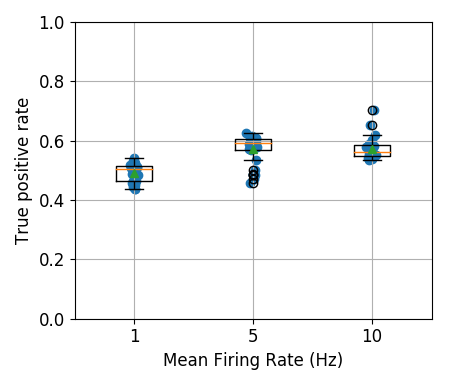
\includegraphics[width=0.5\linewidth]{figures/simulated_oasis_tp_paper.png}
  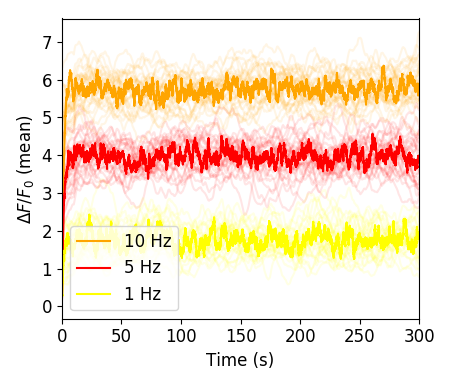
\includegraphics[width=0.5\linewidth]{figures/mean_fluorescence_comparison.png}
  \caption{(left) The spike inference true positive rate when applied to 30 traces created using simulated spike trains with mean firing rates of 1, 5, and 10 Hz. (right) The mean $\Delta F/F_0$ across those 30 traces for each frequency.}
  \label{}
\end{figure}




\end{document}
